\documentclass[]{beamer}
\usepackage[T1]{fontenc}
\usepackage[utf8]{inputenc}
\usepackage{lmodern}
\usepackage[italian]{babel}

\title{Il suono}
\author{\texorpdfstring{Mattia Cozzi\newline\href{mailto:cozzimattia@gmail.com}{\texttt{cozzimattia@gmail.com}}}{Mattia Cozzi}}
\date{a.s.~2023/2024}

%\documentclass[handout]{beamer}     %usare questa classe per generare l'handout
%\usepackage{pgfpages}   %per mostrare più quadri nella stessa pagina
%\pgfpagesuselayout{4 on 1}[a4paper,border shrink=5mm,landscape]
\usetheme{Singapore}
%\useoutertheme[left]{sidebar} %elementi intorno alle diapositive
\setbeamercovered{dynamic} %modifica l'aspetto del testo grigetto delle diapositive future. Argomenti: invisible/transparent/dynamic
\usecolortheme{orchid}
%COLORE PRINCIPALE
\definecolor{marroncino}{RGB}{156, 26, 0} % UBC Blue (primary)
\setbeamercolor{structure}{fg=marroncino} % itemize, enumerate, etc

\theoremstyle{plain}
\newtheorem{teorema}{Teorema}

\usepackage{tikz}


\usepackage{pgf,pgfplots,graphicx}
\usetikzlibrary{angles,quotes,arrows,shapes,decorations.markings}
\pgfplotsset{compat=1.15}
\usepgfplotslibrary{units,fillbetween} % to add units easily to axis



\begin{document}

\begin{frame}
  \titlepage
\end{frame}





\begin{frame}
\frametitle{Contenuti}
\tableofcontents
\end{frame}


\section{Onde sonore}


\begin{frame}
\frametitle{Definizione}
Il suono è un'\alert<1>{onda longitudinale} generata da successive compressioni e rarefazioni del mezzo materiale in cui il suono si propaga.\\\pause~\\La grandezza oscillante sarà la \alert<2>{pressione dell'aria} (oppure, equivalentemente, la sua densità).\\~\\\pause
Essendo un'onda meccanica, il suono non si propaga nel vuoto, ma \alert<3>{richiede un mezzo materiale}.
\begin{center}
\href{gif/suono1.gif}{\beamergotobutton{GIF: Onde sonore 1}}~~~~~~~~~~\href{gif/suono2.gif}{\beamergotobutton{GIF: Onde sonore 2}}
\end{center}
\end{frame}



\begin{frame}
\frametitle{Velocità del suono}
Come tutte le onde ha una certa velocità di propagazione, che \alert{dipende dal mezzo e dalla sua temperatura}.

Ovviamente il suono rimane, in ogni mezzo, molto più lento della luce.\\~

\centering
  \begin{tabular}{c|c}
    \textbf{Mezzo} & \textbf{Velocità} \\\hline\rule{0pt}{3ex}
    Aria a $ 0\,{}^\circ C $ & $ 331 \, \frac{m}{s} $ \\\rule{0pt}{3ex}
    Aria a $ 20 \,{}^\circ C$ & $ 343 \, \frac{m}{s} $ \\\rule{0pt}{3ex}
    Acqua a $ 20\,{}^\circ C $ & $ 1484 \, \frac{m}{s} $ \\\rule{0pt}{3ex}
    Ferro & $ 5130 \, \frac{m}{s} $\\
  \end{tabular}
\end{frame}



\begin{frame}
\frametitle{Esercizio}
\begin{exampleblock}{Distanza dagli altoparlanti}
\small{A un concerto tenuto in uno stadio, l'ultima fila di spettatori si trova a $ 150 \, m $ dagli altoparlanti.

Quale è il ritardo $ \Delta t $ con cui la musica giunge a questi spettatori?\hspace*{\fill}[$ 4,41 \times 10^{-1} \, s $]}
\end{exampleblock}
\end{frame}

% \begin{frame}
% \frametitle{Esempio (1)}
% \begin{exampleblock}{Distanza di un tuono}
% a
% \end{exampleblock}\pause
% ~\\
% b
% \end{frame}



\begin{frame}
\frametitle{Emissione e ricezione umana (1)}
Gli esseri umani emettono suoni utilizzando tutto l'apparato respiratorio, in particolar modo le \alert{corde vocali}, piccole membrane tese all'imbocco della trachea che vibrano per effetto dell'aria emessa dai polmoni.\visible<2>{
\begin{figure}
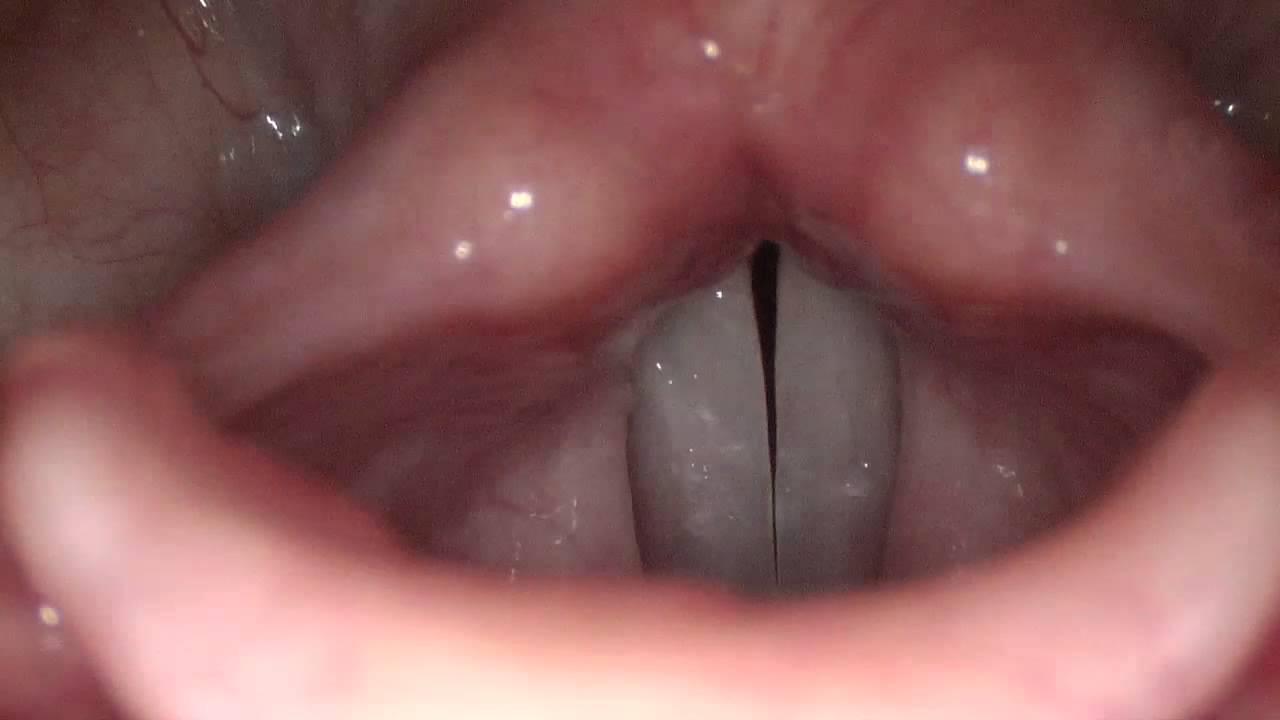
\includegraphics[width=.6\columnwidth]{img/cordevocali.jpg}

\href{video/Cordevocali.mp4}{\beamergotobutton{Video: Corde vocali durante il canto}}
\end{figure}}
\end{frame}


\begin{frame}
\frametitle{Emissione e ricezione umana (2)}
Gli esseri umani sentono i suoni grazie ad una membrana posta nell'orecchio, il \alert{timpano}, che vibra con l'aria e trasmette il movimento agli ossicini dell'orecchio medio (martello, incudine, staffa), che a loro volta muovono la chiocciola, una struttura a spirale piena di liquido. Le oscillazioni del liquido eccitano delle terminazioni nervose che portano il segnale al cervello.\visible<2>{
\begin{figure}
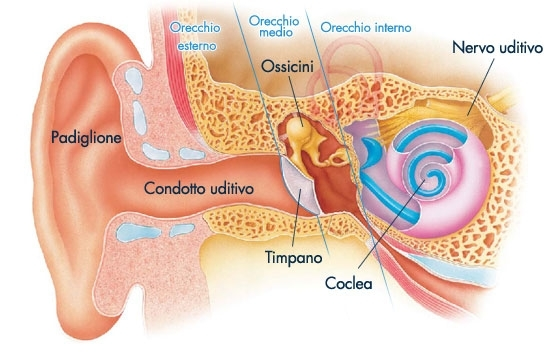
\includegraphics[width=.4\columnwidth]{img/orecchio.jpg}

\href{video/Udito.mp4}{\beamergotobutton{Video: L'udito umano}}
\end{figure}}
\end{frame}

\section{Proprietà}

\begin{frame}
\frametitle{Caratteristiche del suono}
Distinguiamo i suoni in base a tre caratteristiche:
\begin{itemize}
  \item l'\alert<1>{altezza}, che dipende dalla frequenza del suono e distingue un suono grave da uno acuto;\pause
  \item l'\alert<2>{intensità}, che dipende dall'ampiezza dell'onda e distingue un suono a basso volume da uno ad alto volume;\pause
  \item il \alert<3>{timbro}, che dipende dalla particolare forma dell'onda periodica e distingue una voce da un'altra.
\end{itemize}
\begin{columns}
\begin{column}{0.3\textwidth}
\visible<1->{\begin{figure}
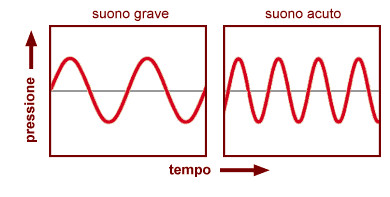
\includegraphics[width=\columnwidth]{img/suono1.jpg}
\end{figure}}
\end{column}
\begin{column}{0.3\textwidth}
\visible<2->{\begin{figure}
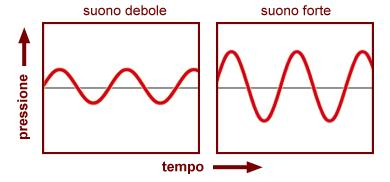
\includegraphics[width=\columnwidth]{img/suono2.jpg}
\end{figure}}
\end{column}
\begin{column}{0.3\textwidth}
\visible<3->{\begin{figure}
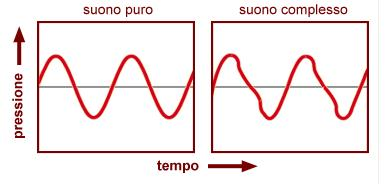
\includegraphics[width=\columnwidth]{img/suono3.jpg}
\end{figure}}
\end{column}
\end{columns}
\end{frame}


\begin{frame}
\frametitle{Strumenti musicali}
Ogni strumento musicale, in base al modo in cui emette il suono (corde vibranti, membrane vibranti, piatti, ecc.) ha un sua sua forma d'onda peculiare e di conseguenza un timbro specifico.\\~\\

Ad ogni nota corrisponde una esatta frequenza del suono emesso.\\~\\
\begin{center}
\href{video/Gopro1.mp4}{\beamergotobutton{Video: Chitarra 1}}~~~~~~~~~~~~~~~\href{video/Gopro2.mp4}{\beamergotobutton{Video: Chitarra 2}}
\end{center}
\end{frame}


\section{Limiti}

\begin{frame}
\frametitle{Limiti di udibilità}
\begin{block}{Limiti di udibilità}
Per essere udibile, un suono deve avere una frequenza compresa tra $ 20 \, Hz $ e $ 20 \, 000 \, Hz $.
\end{block}
Se:\begin{itemize}
  \item $ f < 20 \, Hz $ abbiamo gli \emph{infrasuoni}; 
  \item $ f > 20\, 000 \, Hz $ abbiamo gli \emph{ultrasuoni}.
\end{itemize}\pause

~

Ricordiamo che:
\begin{center}
$ v = \lambda f $
\end{center}
\end{frame}


\begin{frame}
\frametitle{Frequenze percepite (blu) ed emesse (rosso)}
\begin{figure}
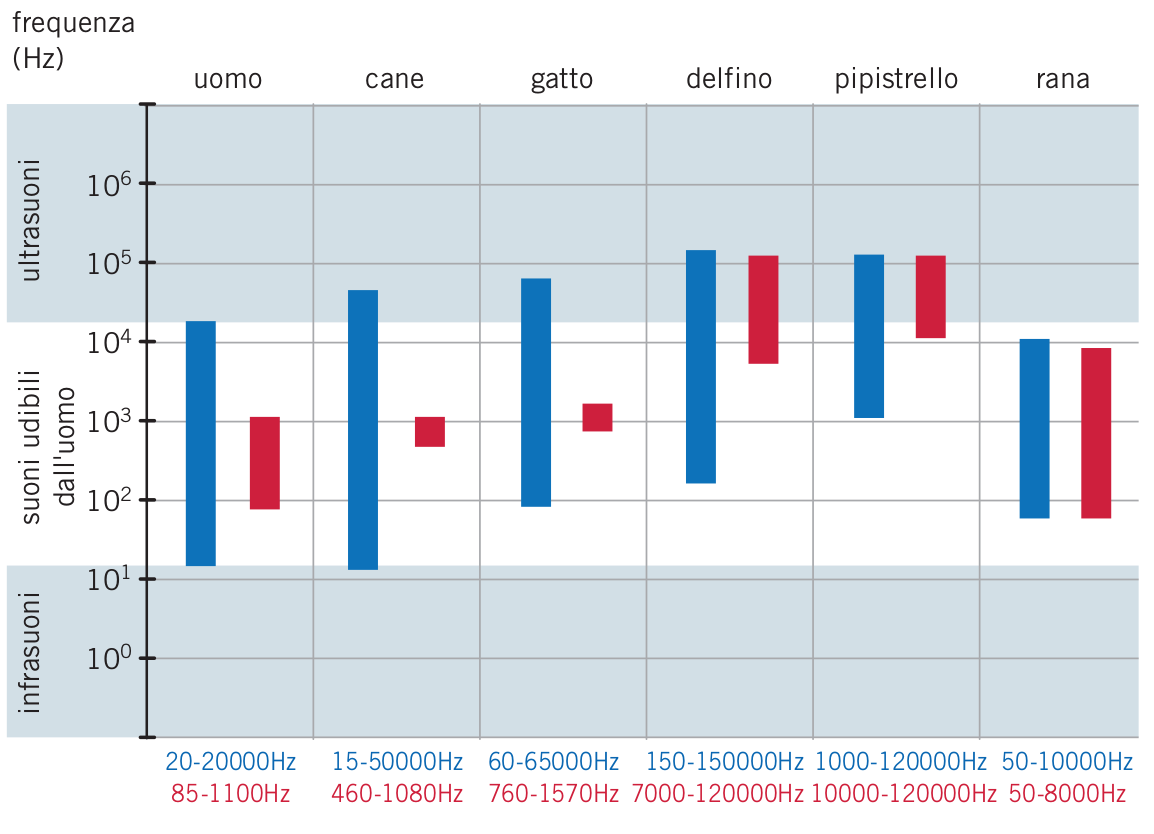
\includegraphics[width=.8\columnwidth]{img/suoni.png}
\end{figure}
\end{frame}



\begin{frame}
\frametitle{Esercizio}
\begin{exampleblock}{Udibilità di un suono}
\small{Un'onda sonora ha una lunghezza d'onda $ \lambda = 34,0 \, m $. 

È udibile in aria? Perché?}
\end{exampleblock}
\end{frame}

\section{Eco}

\begin{frame}
\frametitle{L'eco}
L'eco è dovuta al fatto che le onde sonore vengono \alert<1>{riflesse} da un ostacolo.\\~\\
\begin{figure}
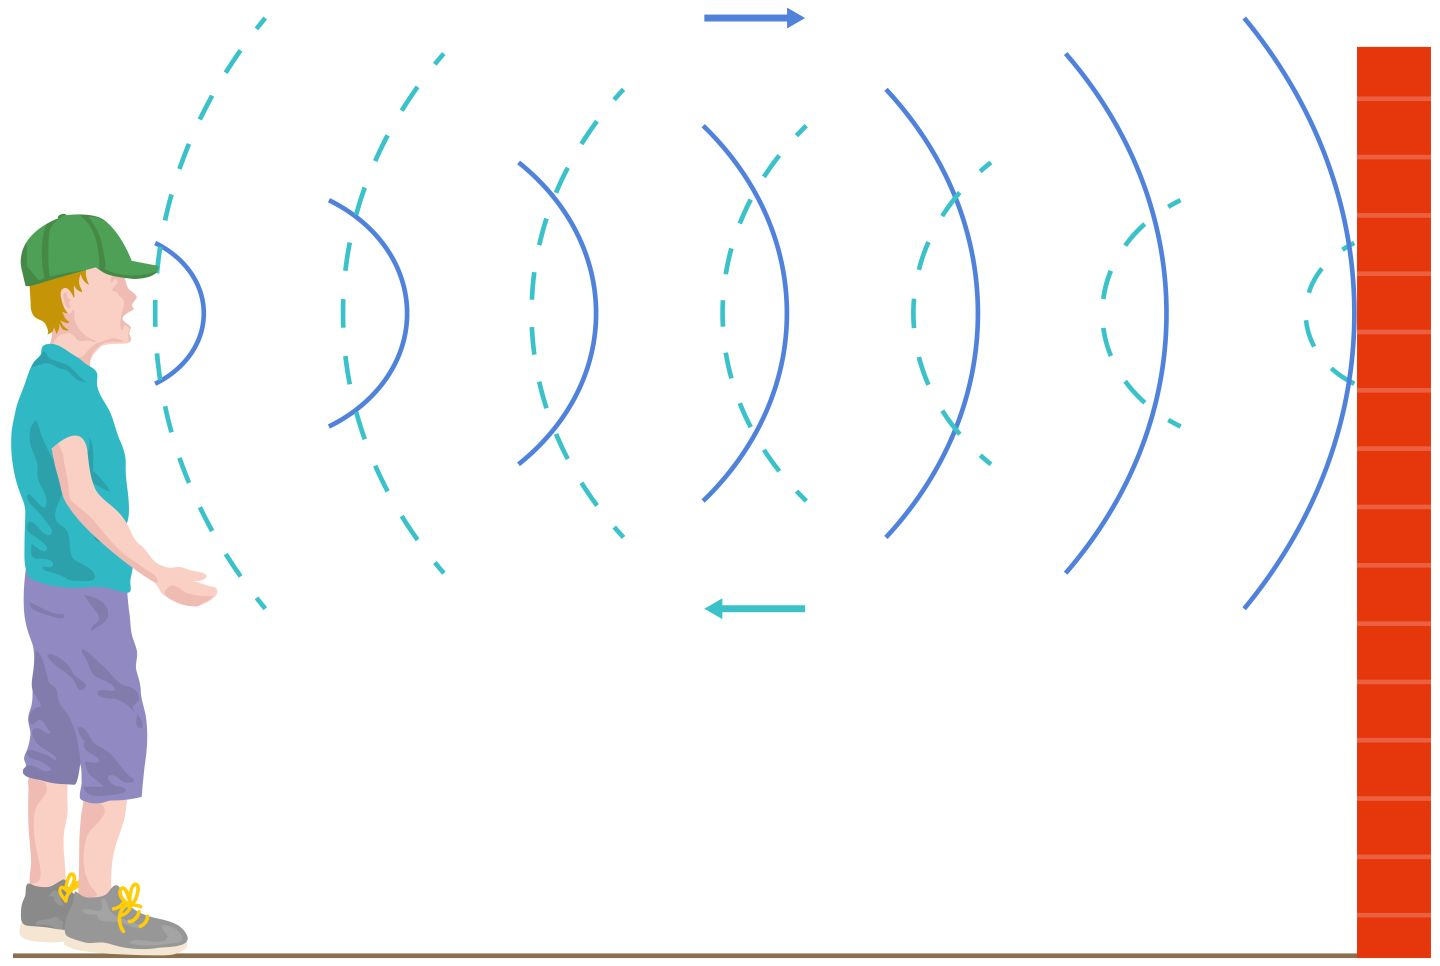
\includegraphics[width=.6\columnwidth]{img/eco.jpg}
\end{figure}
\end{frame}
\begin{frame}
\frametitle{Distanza minima}
Sappiamo che:
\begin{itemize}
  \item il suono viaggia nell'aria a circa $ 340 \, \frac{m}{s} $;\pause
  \item l'orecchio umano percepisce due suoni in modo distinto se essi sono intervallati da almeno $ \frac{1}{10} $ di secondo;\pause
  \item in $ \frac{1}{10} $ di secondo un'onda sonora percorre $ 34\, m $.\pause
\end{itemize}

~

Perché si percepisca un'eco, \alert{è necessario un ostacolo posto ad almeno $ 17 \, m $} (cioè un totale di $ 34 \, m $ tra andata e ritorno).\pause

~

Per distanze (e tempi) inferiori si parla invece di \emph{riverbero}.
\end{frame}

\begin{frame}
  \frametitle{Utilizzi dell'eco}
  \begin{columns}
    \begin{column}{0.3\textwidth}
      \begin{figure}
        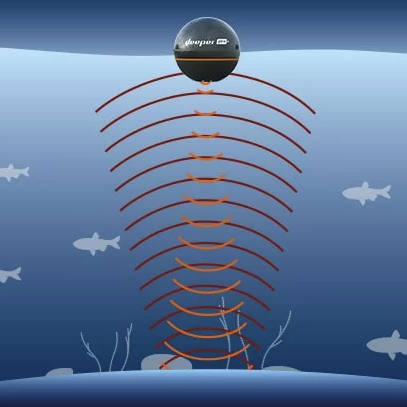
\includegraphics[width=\columnwidth]{img/sonar.png}
        
        Sonar
        
        ~
      \end{figure}
    \end{column}
    \begin{column}{0.3\textwidth}
      \visible<2-3>{\begin{figure}
        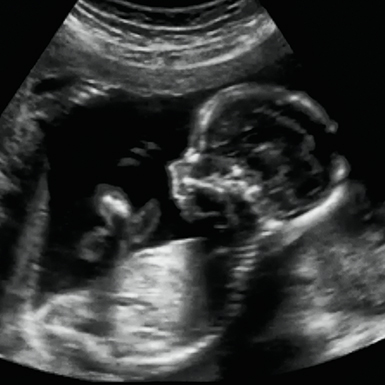
\includegraphics[width=\columnwidth]{img/ecografia.jpg}
        
        Ecografia
        
        ~
      \end{figure}
      }
    \end{column}
    \begin{column}{0.3\textwidth}
      \visible<3>{\begin{figure}
        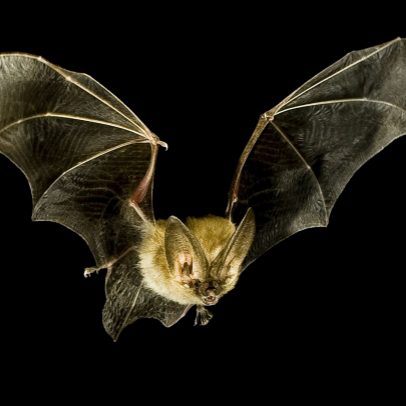
\includegraphics[width=\columnwidth]{img/pipistrello.jpg}
        
        Pipistrelli, delfini e balene
      \end{figure}
      }
    \end{column}
  \end{columns}
\end{frame}

\section{Doppler}

\begin{frame}
\frametitle{Fenomeno}
Studiamo ora l'effetto sonoro che udiamo quando ci passa di fianco un'ambulanza o un'auto che sta suonando il clacson. \href{video/Dopplerauto.mp4}{\beamergotobutton{Video: Clacson}}\pause

~

È conseguenza del fatto che la sorgente (auto) e il ricevitore (noi) sono \alert<2>{in moto l'uno rispetto all'altro}.

\visible<2>{
\begin{columns}
    \begin{column}{0.4\textwidth}
      \begin{figure}
        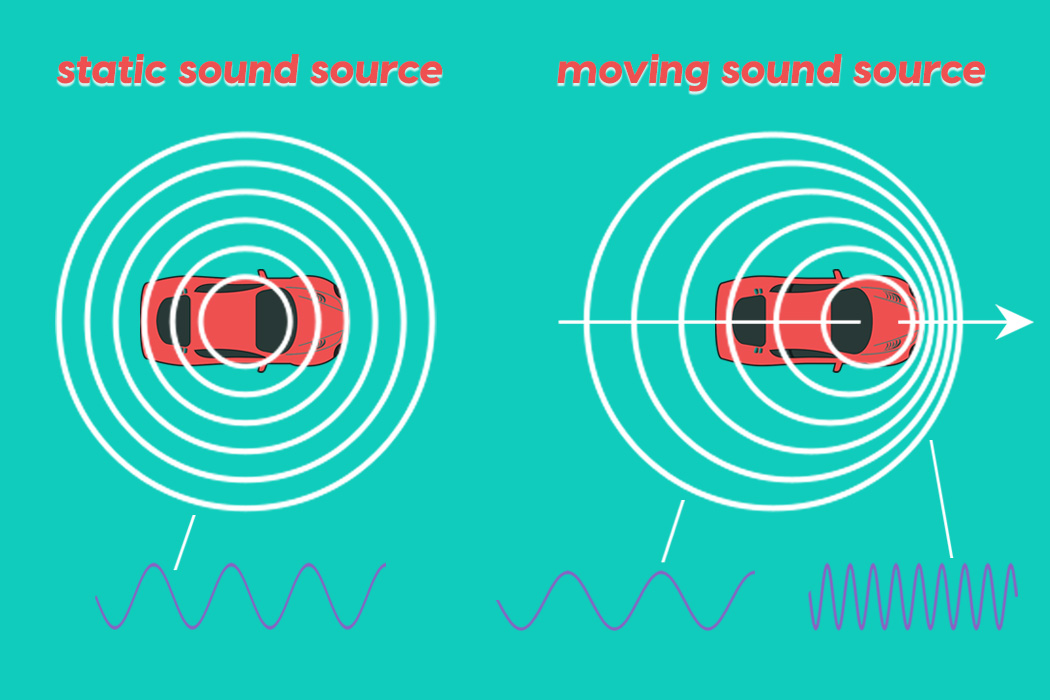
\includegraphics[width=\columnwidth]{img/doppler.jpg}
      \end{figure}
    \end{column}
    \begin{column}{0.4\textwidth}
      \begin{figure}
        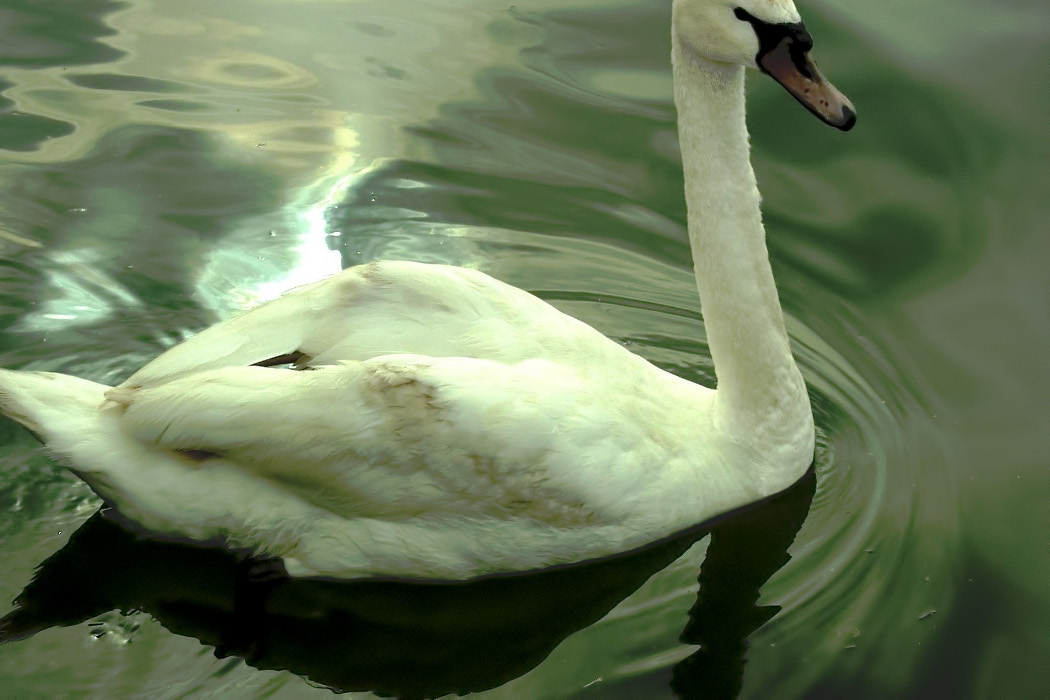
\includegraphics[width=\columnwidth]{img/cigno.jpg}
      \end{figure}
    \end{column}
  \end{columns}
}
\end{frame}


\begin{frame}
\frametitle{Effetto Doppler}
\begin{block}{Effetto Doppler}
La frequenza di un'onda periodica, rilevata da un rilevatore in moto rispetto alla sorgente, è diversa da quella di emissione.
\end{block}\pause~\\

Abbiamo due casi possibili:
\begin{itemize}
  \item se sorgente e rilevatore \alert<2>{si allontanano}, la frequenza rilevata $ f' $ sarà \alert<2>{minore} di quella emessa $ f $;\pause
  \item se \alert<3>{si avvicinano}, la frequenza rilevata $ f' $ sarà \alert<3>{maggiore} di quella emessa $ f $;\pause
 \end{itemize}
\end{frame}




\begin{frame}
  \frametitle{Utilizzi dell'effetto Doppler}
  \begin{columns}
    \begin{column}{0.3\textwidth}
      \begin{figure}
        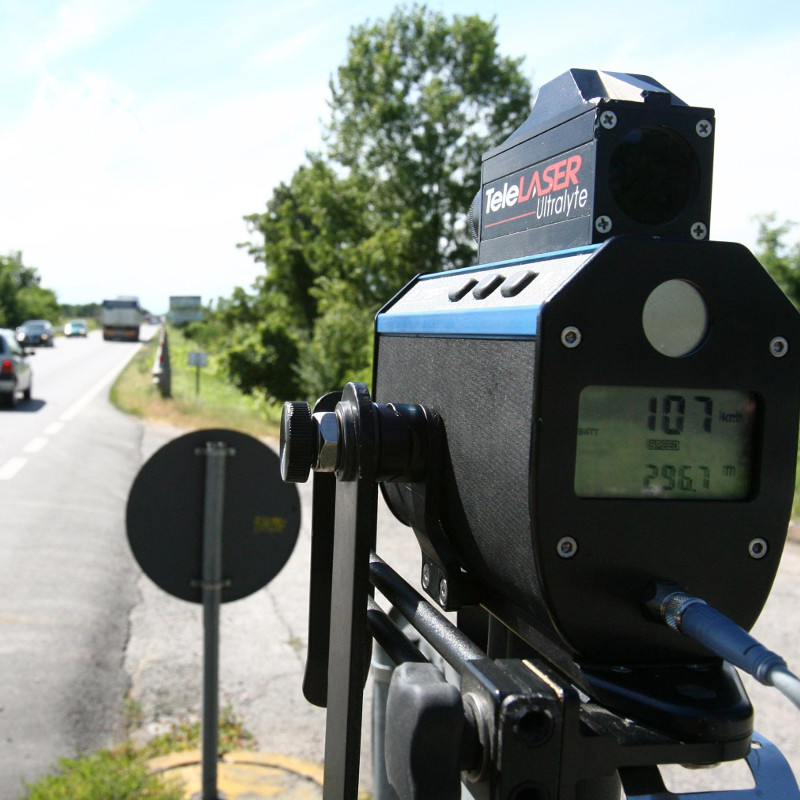
\includegraphics[width=\columnwidth]{img/autovelox.jpg}
        
        Autovelox\\(alcuni modelli)
      \end{figure}
    \end{column}
    \begin{column}{0.3\textwidth}
      \visible<2-3>{\begin{figure}
        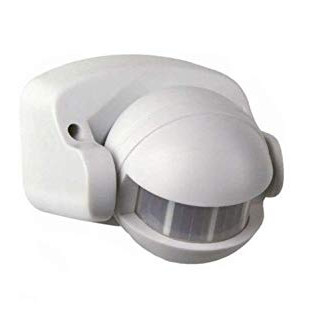
\includegraphics[width=\columnwidth]{img/sensore.jpg}
        
        Sensori di movimento
      \end{figure}
      }
    \end{column}
    \begin{column}{0.3\textwidth}
      \visible<3>{\begin{figure}
        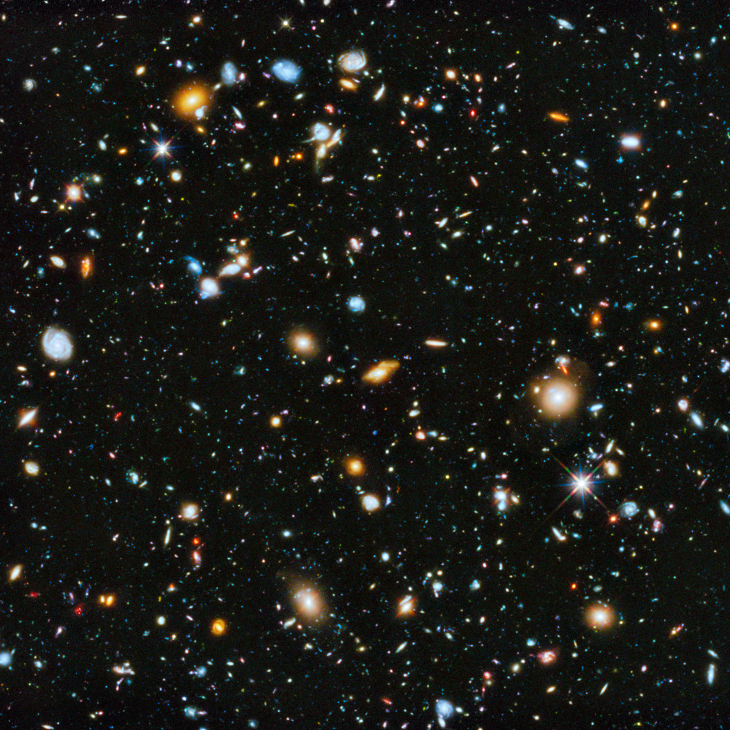
\includegraphics[width=\columnwidth]{img/hubbledeepfield.jpg}
        
        Allontanamento delle galassie
      \end{figure}
      }
    \end{column}
  \end{columns}
\end{frame}


\end{document}
